\subsection*{XGBoost on CIC-IDS2017 in NIDS pipeline outputs}
\begin{figure}[H]
     \centering
     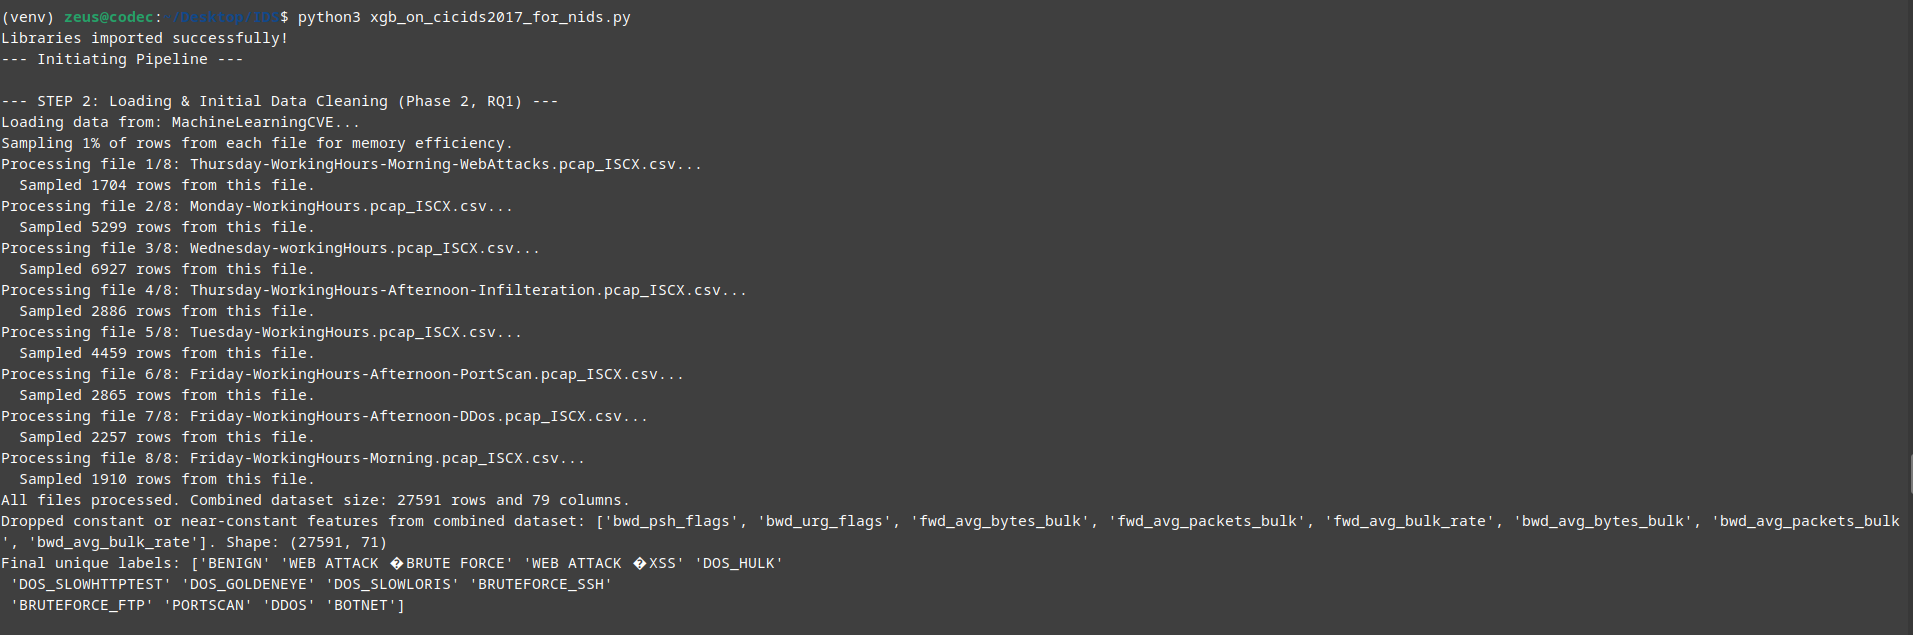
\includegraphics[width=0.75\textwidth]{assets/figures/outputs/1.png}
     %caption{whatweb output}
     %\label{fig:whatwebb} 
 \end{figure}
 
 \begin{figure}[H]
     \centering
     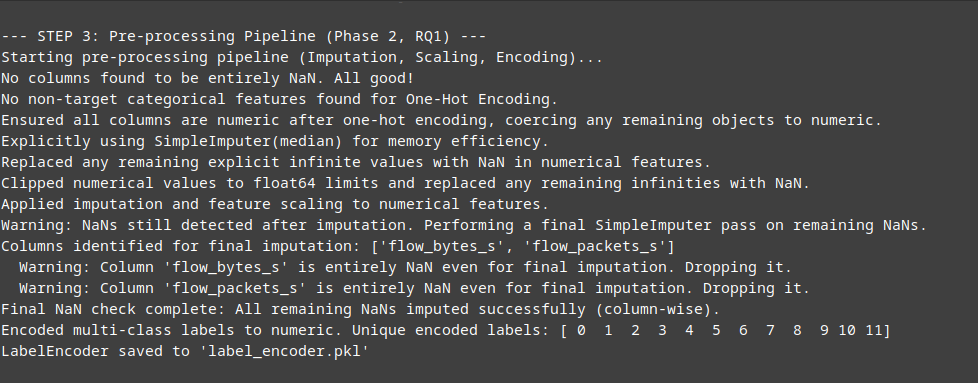
\includegraphics[width=0.75\textwidth]{assets/figures/outputs/2.png}
     %caption{whatweb output}
     %\label{fig:whatwebb} 
 \end{figure}
 
 \begin{figure}[H]
     \centering
     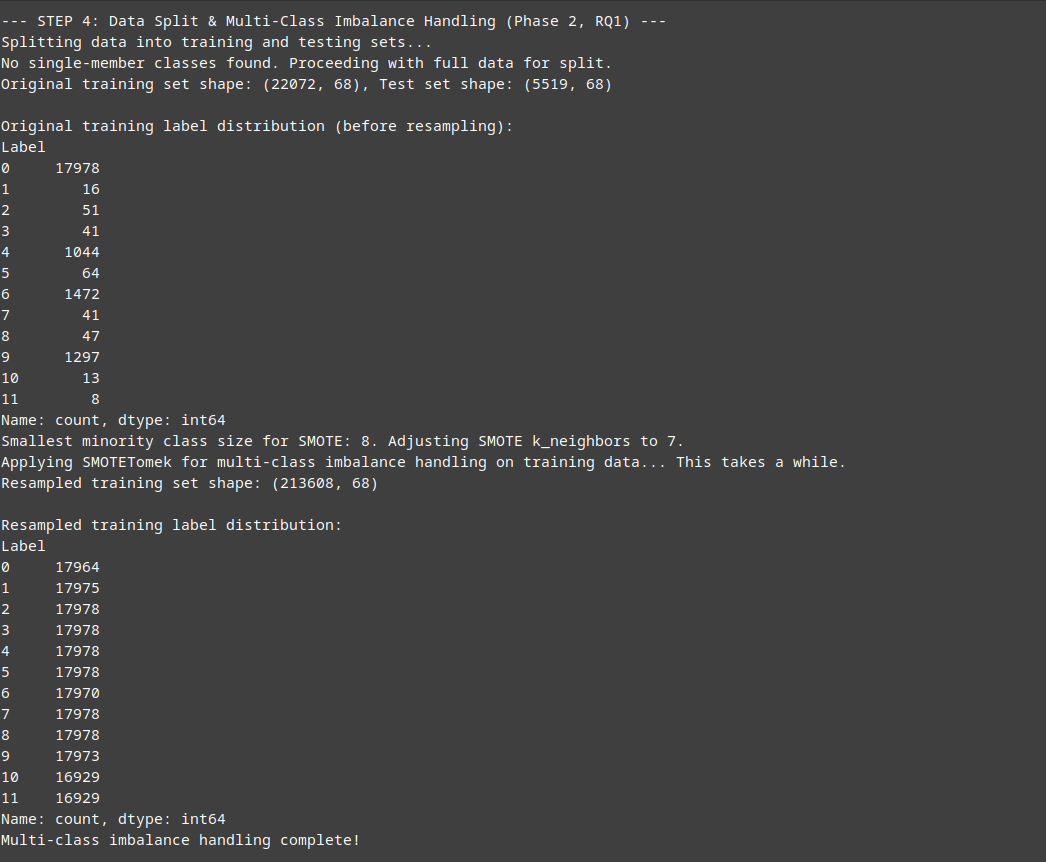
\includegraphics[width=0.75\textwidth]{assets/figures/outputs/3.png}
     %caption{whatweb output}
     %\label{fig:whatwebb} 
 \end{figure}
 
 \begin{figure}[H]
     \centering
     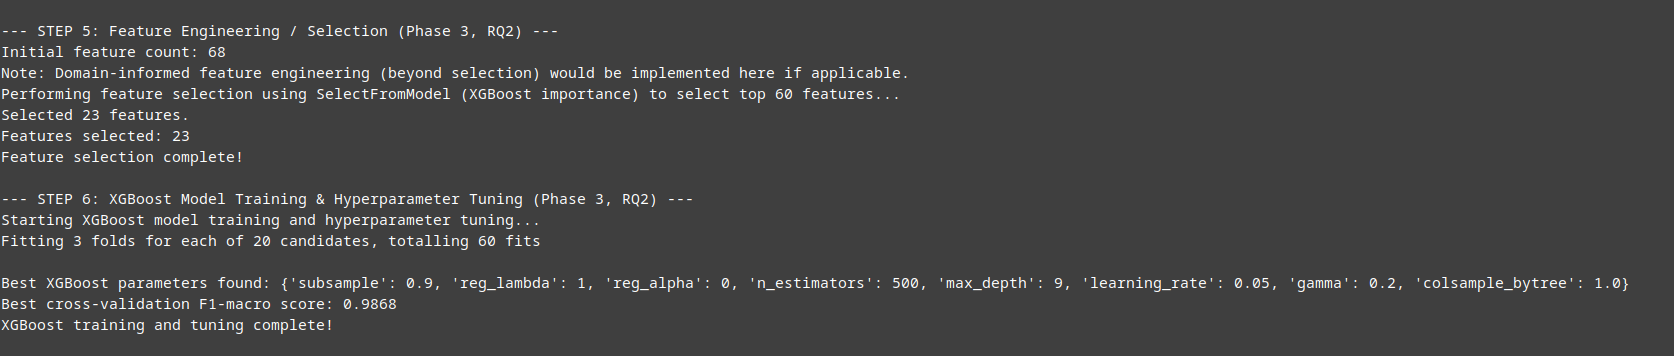
\includegraphics[width=0.75\textwidth]{assets/figures/outputs/4.png}
     %caption{whatweb output}
     %\label{fig:whatwebb} 
 \end{figure}
 
 \begin{figure}[H]
     \centering
     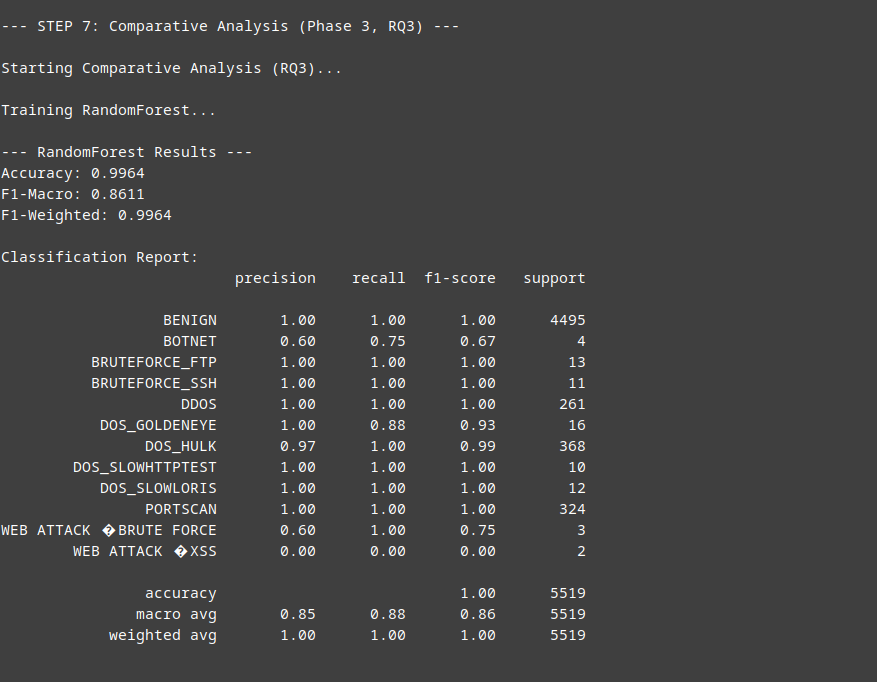
\includegraphics[width=0.75\textwidth]{assets/figures/outputs/5.png}
     %caption{whatweb output}
     %\label{fig:whatwebb} 
 \end{figure}
 
 \begin{figure}[H]
     \centering
     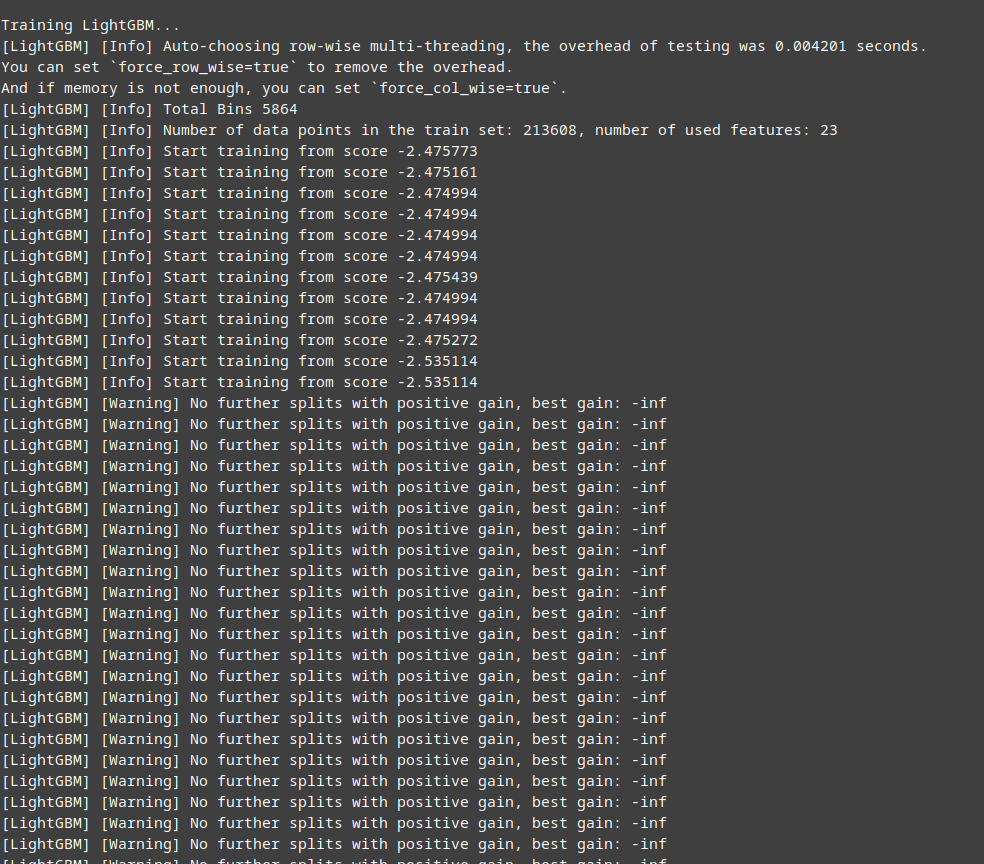
\includegraphics[width=0.75\textwidth]{assets/figures/outputs/6.png}
     %caption{whatweb output}
     %\label{fig:whatwebb} 
 \end{figure}
 
 \begin{figure}[H]
     \centering
     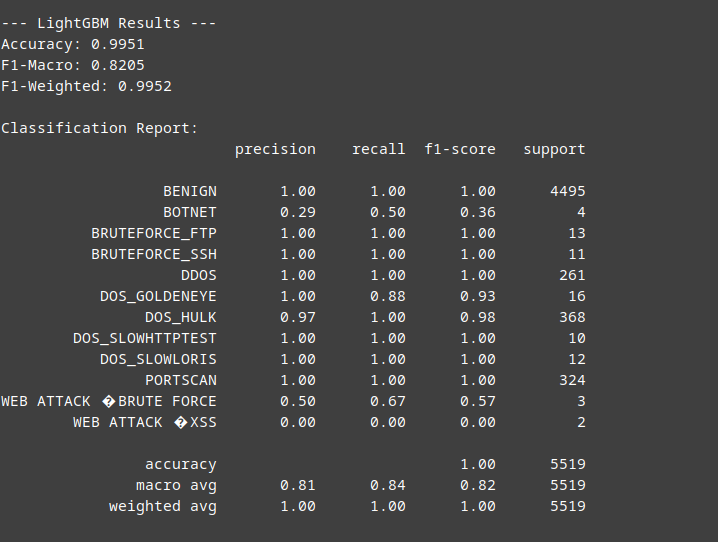
\includegraphics[width=0.75\textwidth]{assets/figures/outputs/7.png}
     %caption{whatweb output}
     %\label{fig:whatwebb} 
 \end{figure}
 
 \begin{figure}[H]
     \centering
     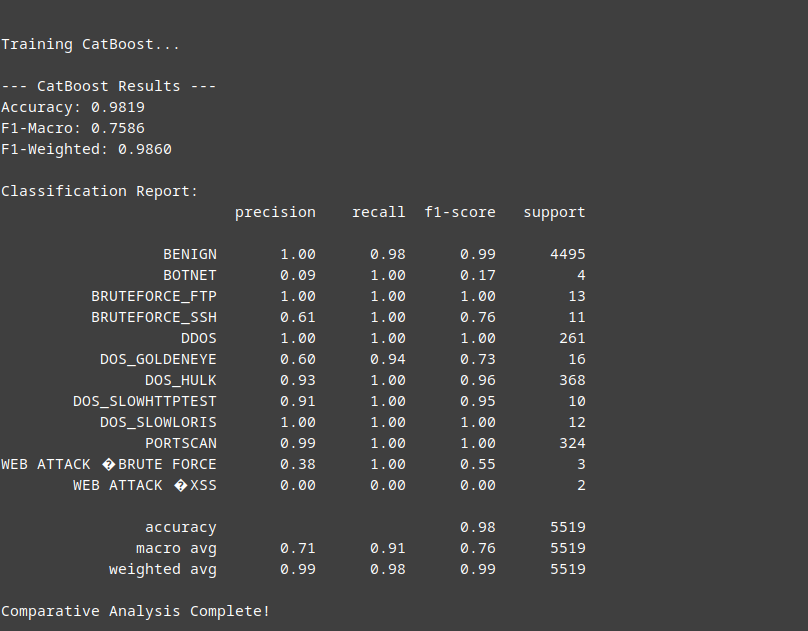
\includegraphics[width=0.75\textwidth]{assets/figures/outputs/8.png}
     %caption{whatweb output}
     %\label{fig:whatwebb} 
 \end{figure}
 
 \begin{figure}[H]
     \centering
     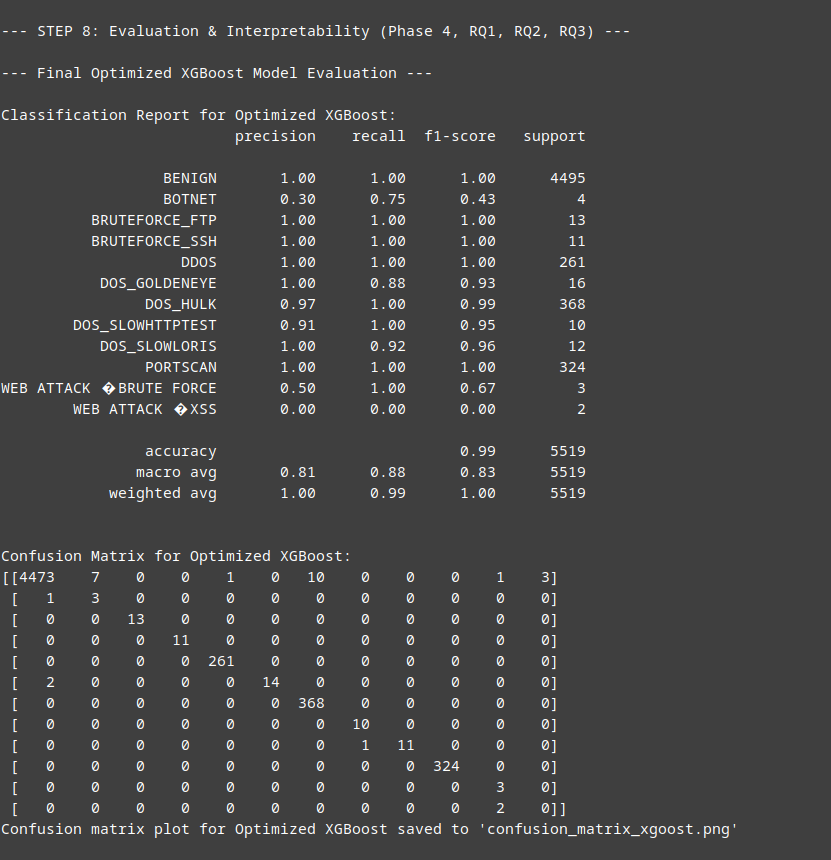
\includegraphics[width=0.75\textwidth]{assets/figures/outputs/9.png}
     \%caption{whatweb output}
     %\label{fig:whatwebb} 
 \end{figure}
 
 \begin{figure}[H]
     \centering
     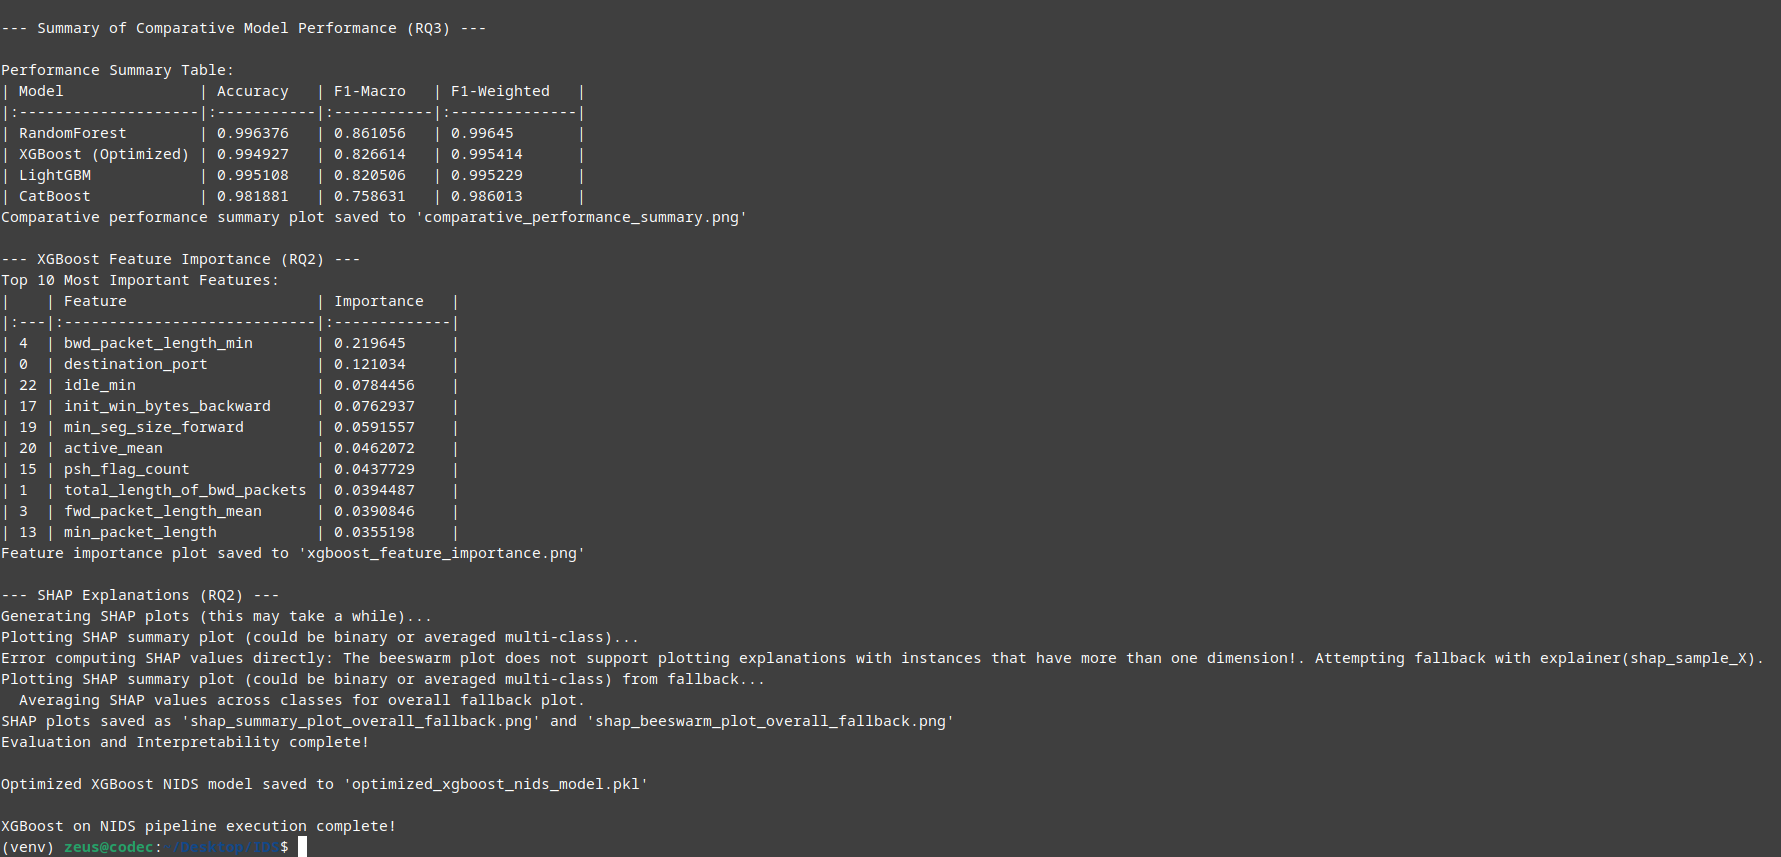
\includegraphics[width=0.75\textwidth]{assets/figures/outputs/10.png}
     %caption{whatweb output}
     %\label{fig:whatwebb} 
 \end{figure}

% Define column types with wrapping
\newcolumntype{L}[1]{>{\raggedright\arraybackslash}p{#1}}
\newcolumntype{C}[1]{>{\centering\arraybackslash}p{#1}}
\newcolumntype{R}[1]{>{\raggedleft\arraybackslash}p{#1}}

\begin{longtable}{|L{6cm}|C{2cm}|C{2.5cm}|C{3cm}|C{2cm}|}
\caption{Dataset Features: Data Types, Null Values, Memory Usage, and Associated Commands}\label{tab:info} \\
\hline
\textbf{Feature} & \textbf{Data Type} & \textbf{Null Values} & \textbf{Memory Usage (RAM)} & \textbf{Command} \\
\hline
\endfirsthead

\hline
\textbf{Feature} & \textbf{Data Type} & \textbf{Null Values} & \textbf{Memory Usage (RAM)} & \textbf{Command} \\
\hline
\endhead

DestinationPort & int64 & 0 & 581MB & .info() \\ \hline 
Duration & float64 & 0 & 581MB & .info() \\ \hline 
Flow\textunderscore ID & int64 & 0 & 581MB & .info() \\ \hline 
Label & object & 2030 NaNs & 2.9MB & .info() \\ \hline 
Month & int64 & 0 & 581MB & .info() \\ \hline 
New\textunderscore Connections & int64 & 0 & 581MB & .info() \\ \hline 
Packet\textunderscore Direction & object & 0 & 581MB & .info() \\ \hline 
Packets\textunderscore In\textunderscore PerIOD & int64 & 0 & 581MB & .info() \\ \hline 
Packets\textunderscore Out\textunderscore PerIOD & int64 & 0 & 581MB & .info() \\ \hline 
Packet\textunderscore Size & int64 & 0 & 581MB & .info() \\ \hline 
Protocol & object & 0 & 581MB & .info() \\ \hline 
Source\textunderscore Flags & int64 & 0 & 581MB & .info() \\ \hline 
SourcePort & int64 & 0 & 581MB & .info() \\ \hline 
Total\textunderscore Flow\textunderscore Packet\textunderscore Count & int64 & 0 & 581MB & .info() \\ \hline 
Total\textunderscore Packet\textunderscore Length & float64 & 0 & 581MB & .info() \\ \hline 
Total\textunderscore FlowBytes\textunderscore Length & float64 & 0 & 581MB & .info() \\ \hline 
Year & int64 & 0 & 581MB & .info() \\ \hline 
FTP\textunderscore ORIGINALFERETSIZE & int64 & 0 & 581MB & .info() \\ \hline 
HTTPMethods & object & 0 & 581MB & .info() \\ \hline 
HTTPRequest\textunderscore Referer & object & 0 & 581MB & .info() \\ \hline 
HTTPRequest\textunderscore ResponseCode & object & 0 & 581MB & .info() \\ \hline 
HTTPRequest\textunderscore UserAgent & object & 0 & 581MB & .info() \\ \hline 
HTTPResponse\textunderscore Code & object & 0 & 581MB & .info() \\ \hline 
JSON\textunderscore JSON & object & 0 & 581MB & .info() \\ \hline 
Packet\textunderscore Sequence\textunderscore Number& int64 & 0 & 581MB & .info() \\ \hline 
SFTP\textunderscore OriginalFERETSIZE & int64 & 0 & 581MB & .info() \\ \hline 
SSLVersion & object & 0 & 581MB & .info() \\ \hline 
SSHCommand\textunderscore ID & int64 & 0 & 581MB & .info() \\ \hline 
SSHVersion & object & 0 & 581MB & .info() \\ \hline 
TLSTicketLifetime & float64 & 0 & 581MB & .info() \\ \hline 
FTPDataTransferSize & int64 & 0 & 581MB & .info() \\ \hline 
FTPCommandID & int64 & 0 & 581MB & .info() \\ \hline 
DNSQryName & object & 0 & 581MB & .info() \\ \hline 
DNSRR & object & 0 & 581MB & .info() \\ \hline 
Dst\textunderscore Land & object & 0 & 581MB & .info() \\ \hline 
Dst\textunderscore Lon & float64 & 0 & 581MB & .info() \\ \hline 
Dst\textunderscore Src\textunderscore win\textunderscore ratio & float64 & 0 & 581MB & .info() \\ \hline 
Dst\textunderscore Weird\textunderscore flag\textunderscore freq & float64 & 0 & 581MB & .info() \\ \hline 
Dst\textunderscore WinSize & float64 & 0 & 581MB & .info() \\ \hline 
Dst\textunderscore Mean\textunderscore PacketSize & float64 & 0 & 581MB & .info() \\ \hline 
Dst\textunderscore Median\textunderscore PacketSize & float64 & 0 & 581MB & .info() \\ \hline 
Dst\textunderscore Min\textunderscore PacketSize & float64 & 0 & 581MB & .info() \\ \hline 
Dst\textunderscore Max\textunderscore PacketSize & float64 & 0 & 581MB & .info() \\ \hline 
Dst\textunderscore Skew\textunderscore PacketSize & float64 & 0 & 581MB & .info() \\ \hline 
Dst\textunderscore Src\textunderscore connect\textunderscore ratio & float64 & 0 & 581MB & .info() \\ \hline 
Dst\textunderscore Src\textunderscore count\textunderscore rate & float64 & 0 & 581MB & .info() \\ \hline 
Dst\textunderscore IP\textunderscore packets\textunderscore count & int64 & 0 & 581MB & .info() \\ \hline 
Dst\textunderscore Port\textunderscore packets\textunderscore count& int64 & 0 & 581MB & .info() \\ \hline 
Dst\textunderscore PortFrac & float64 & 0 & 581MB & .info() \\ \hline 
Dst\textunderscore PortZeroByteFraction& float64 & 0 & 581MB & .info() \\ \hline 
Dst\textunderscore PKTS & int64 & 0 & 581MB & .info() \\ \hline 
Dst\textunderscore TotalPacketLength & float64 & 0 & 581MB & .info() \\ \hline 
Dst\textunderscore IP\textunderscore ZeroByteRate & float64 & 0 & 581MB & .info() \\ \hline 
Dst\textunderscore Port\textunderscore ZeroByteRate & float64 & 0 & 581MB & .info() \\ \hline 
Dst\textunderscore TotalByteRate & float64 & 0 & 581MB & .info() \\ \hline 
DstByteRateFrac & float64 & 0 & 581MB & .info() \\ \hline 
DstUDPByteRateFrac & float64 & 0 & 581MB & .info() \\ \hline 
Dst\textunderscore ZeroByteFraction & float64 & 0 & 581MB & .info() \\ \hline 
Dst\textunderscore ZeroByteRate & float64 & 0 & 581MB & .info() \\ \hline 
DstBytesPerIPsec & float64 & 0 & 581MB & .info() \\ \hline 
DstBytesPerPkts & float64 & 0 & 581MB & .info() \\ \hline 
Dst\textunderscore TCP\textunderscore Mean\textunderscore PacketSize& float64 & 0 & 581MB & .info() \\ \hline 
Dst\textunderscore TCP\textunderscore Median\textunderscore PacketSize& float64 & 0 & 581MB & .info() \\ \hline 
Dst\textunderscore TCP\textunderscore Min\textunderscore PacketSize& float64 & 0 & 581MB & .info() \\ \hline 
Dst\textunderscore TCP\textunderscore Max\textunderscore PacketSize& float64 & 0 & 581MB & .info() \\ \hline 
Dst\textunderscore TCP\textunderscore Skew\textunderscore PacketSize& float64 & 0 & 581MB & .info() \\ \hline 
Dst\textunderscore UDP\textunderscore Mean\textunderscore PacketSize& float64 & 0 & 581MB & .info() \\ \hline 
Dst\textunderscore UDP\textunderscore Median\textunderscore PacketSize& float64 & 0 & 581MB & .info() \\ \hline 
Dst\textunderscore UDP\textunderscore Min\textunderscore PacketSize& float64 & 0 & 581MB & .info() \\ \hline 
Dst\textunderscore UDP\textunderscore Max\textunderscore PacketSize& float64 & 0 & 581MB & .info() \\ \hline 
Dst\textunderscore UDP\textunderscore Skew\textunderscore PacketSize& float64 & 0 & 581MB & .info() \\ \hline 
FailedLogins & int64 & 0 & 581MB & .info() \\ \hline 
FlowBitsPerSec & float64 & 0 & 581MB & .info() \\ \hline 
HTTPTransferSize & int64 & 6589 NaNs & 581MB & .info() \\ \hline 
Month\textunderscore of\textunderscore the\textunderscore year & object & 0 & 581MB & .info() \\ \hline 
SFTP\textunderscore RegularEXP\textunderscore PERMSTATE& int64 & 0 & 581MB & .info() \\ \hline 
SRC\textunderscore IFACE & object & 0 & 581MB & .info() \\ \hline 
TotalDNS\textunderscore Msg & int64 & 0 & 581MB & .info() \\ \hline 
Src\textunderscore Latitude & float64 & 0 & 581MB & .info() \\ \hline 
Src\textunderscore Latitude\textunderscore ToInt & int64 & 0 & 581MB & .info() \\ \hline 
Src\textunderscore Lon & float64 & 0 & 581MB & .info() \\ \hline 
Src\textunderscore Lon\textunderscore ToInt & int64 & 0 & 581MB & .info() \\ \hline 
Src\textunderscore Land & object & 0 & 581MB & .info() \\ \hline 
Src\textunderscore Mean\textunderscore PacketSize & float64 & 0 & 581MB & .info() \\ \hline 
Src\textunderscore Median\textunderscore PacketSize & float64 & 0 & 581MB & .info() \\ \hline 
Src\textunderscore Min\textunderscore PacketSize & float64 & 0 & 581MB & .info() \\ \hline 
Src\textunderscore Max\textunderscore PacketSize & float64 & 0 & 581MB & .info() \\ \hline 
Src\textunderscore Skew\textunderscore PacketSize & float64 & 0 & 581MB & .info() \\ \hline 
Src\textunderscore WinSize & float64 & 0 & 581MB & .info() \\ \hline 
Src\textunderscore IP\textunderscore Address\textunderscore Count & int64 & 0 & 581MB & .info() \\ \hline 
Src\textunderscore IP\textunderscore packets\textunderscore count & int64 & 0 & 581MB & .info() \\ \hline 
Src\textunderscore Port\textunderscore packets\textunderscore count& int64 & 0 & 581MB & .info() \\ \hline 
Src\textunderscore PortFrac & float64 & 0 & 581MB & .info() \\ \hline 
Src\textunderscore PKTS & int64 & 0 & 581MB & .info() \\ \hline 
Src\textunderscore TotalPacketLength & float64 & 0 & 581MB & .info() \\ \hline 
Src\textunderscore TotalByteRate & float64 & 0 & 581MB & .info() \\ \hline 
SrcByteRateFrac & float64 & 0 & 581MB & .info() \\ \hline 
Src\textunderscore TCP\textunderscore Mean\textunderscore PacketSize& float64 & 0 & 581MB & .info() \\ \hline 
Src\textunderscore TCP\textunderscore Median\textunderscore PacketSize& float64 & 0 & 581MB & .info() \\ \hline 
Src\textunderscore TCP\textunderscore Min\textunderscore PacketSize& float64 & 0 & 581MB & .info() \\ \hline 
Src\textunderscore TCP\textunderscore Max\textunderscore PacketSize& float64 & 0 & 581MB & .info() \\ \hline 
Src\textunderscore TCP\textunderscore Skew\textunderscore PacketSize& float64 & 0 & 581MB & .info() \\ \hline 
Src\textunderscore UDP\textunderscore Mean\textunderscore PacketSize& float64 & 0 & 581MB & .info() \\ \hline 
Src\textunderscore UDP\textunderscore Median\textunderscore PacketSize& float64 & 0 & 581MB & .info() \\ \hline 
Src\textunderscore UDP\textunderscore Min\textunderscore PacketSize& float64 & 0 & 581MB & .info() \\ \hline 
Src\textunderscore UDP\textunderscore Max\textunderscore PacketSize& float64 & 0 & 581MB & .info() \\ \hline 
Src\textunderscore UDP\textunderscore Skew\textunderscore PacketSize& float64 & 0 & 581MB & .info() \\ \hline 
TimeHours & float64 & 0 & 581MB & .info() \\ \hline 
Type\textunderscore of\textunderscore DDoS & object & 0 & 581MB & .info() \\ \hline 
UDP\textunderscore MiscellaneousCommands& object & 0 & 581MB & .info() \\ \hline 
Weekdays & object & 0 & 581MB & .info() \\ \hline 
Is\textunderscore Botnet\textunderscore Attribute & object & 0 & 581MB & .info() \\ \hline 
Is\textunderscore Infiltration\textunderscore Attack & object & 0 & 581MB & .info() \\ \hline 
Is\textunderscore DDOS\textunderscore Attack & object & 0 & 581MB & .info() \\ \hline 
Is\textunderscore DoS\textunderscore Attack & object & 0 & 581MB & .info() \\ \hline 
Is\textunderscore Heartbleed\textunderscore Attack & object & 0 & 581MB & .info() \\ \hline 
Is\textunderscore Web\textunderscore Attack & object & 0 & 581MB & .info() \\ \hline 
Weekends & object & 0 & 581MB & .info() \\ \hline 
WeekHourGroups & object & 0 & 581MB & .info() \\ \hline 
Day\textunderscore Occurences & int64 & 0 & 581MB & .info() \\ \hline 
DaylightSavingsTriggerHours & object & 0 & 581MB & .info() \\ \hline 
DST\textunderscore Code & int64 & 0 & 581MB & .info() \\ \hline 
HoursOfDay & object & 0 & 581MB & .info() \\ \hline 
NonDaylightSavingTriggerHours & object & 0 & 581MB & .info() \\ \hline 
Number\textunderscore Of\textunderscore NonWeekDays & int64 & 0 & 581MB & .info() \\ \hline 
SecondsInHour & int64 & 0 & 581MB & .info() \\ \hline 
Weekday\textunderscore Occurences & int64 & 0 & 581MB & .info() \\ \hline 
\end{longtable}


\begin{lstlisting}[caption={Complete pipeline of XGBoost using CIC-IDS2017 in NIDS using Python}, label={lst:python-pipeline}]
# STEP 1: IMPORT LIBRARIES
import pandas as pd
import numpy as np
import glob
import matplotlib.pyplot as plt
import seaborn as sns
from sklearn.model_selection import train_test_split, RandomizedSearchCV
from sklearn.preprocessing import LabelEncoder, StandardScaler

# --- REQUIRED FOR IterativeImputer (as it's experimental) ---
from sklearn.experimental import enable_iterative_imputer
# ---------------------------------------------------------

from sklearn.impute import SimpleImputer, IterativeImputer  # For advanced imputation (RQ1)
from sklearn.metrics import classification_report, confusion_matrix, accuracy_score, f1_score, roc_auc_score, \
precision_recall_fscore_support
from sklearn.ensemble import RandomForestClassifier  # For comparative analysis (RQ3)
import xgboost as xgb  # For core model (RQ1, RQ2, RQ3)
import lightgbm as lgb  # For comparative analysis (RQ3)
import catboost as cb  # For comparative analysis (RQ3)
import shap  # For interpretability
from imblearn.over_sampling import SMOTE, ADASYN  # For multi-class oversampling strategies (RQ1)
from imblearn.combine import SMOTETomek  # For robust oversampling + undersampling (RQ1)
from imblearn.pipeline import Pipeline as ImbPipeline  # For robust pre-processing pipeline
from sklearn.feature_selection import SelectFromModel  # For feature selection (RQ2)
import joblib
import warnings
import gc  # For garbage collection

warnings.filterwarnings('ignore')  # Suppress warnings for cleaner output, but be cautious in real analysis

print("Libraries imported successfully!")


# ---
# Phase 2 & 3: Data Acquisition and Pre-processing & Model Development & Experimentation
# This section covers loading, initial cleaning, advanced pre-processing,
# data splitting, imbalance handling, feature selection, and model training/tuning.

# ---
# STEP 2: LOAD & INITIAL CLEAN DATA (Phase 2, aligns with RQ1)
# This step focuses on loading all CSVs and performing initial, critical cleaning
# to prepare for more advanced pre-processing strategies (aligns with RQ1).

def load_and_initial_clean_data(data_path, sampling_fraction=1.0, random_state=42):  # Added sampling_fraction
"""
Loads all CIC-IDS2017 CSV files from a specified path,
performs initial data cleaning (dropping irrelevant columns,
standardizing missing/infinite values, converting to numeric types),
and retains multi-class labels. This version is optimized for memory.
Includes an option to sample a fraction of the data from each file.
"""
print(f"\n--- STEP 2: Loading & Initial Data Cleaning (Phase 2, RQ1) ---")
print(f"Loading data from: {data_path}...")
if sampling_fraction < 1.0:
print(f"Sampling {sampling_fraction * 100:.0f}% of rows from each file for memory efficiency.")

file_paths = glob.glob(f'MachineLearningCVE/*.csv')  # Ensure this path is correct for your setup
if not file_paths:
raise ValueError(f"No CSV files found in {data_path}. Please check the path.")

full_df = pd.DataFrame()  # Initialize an empty DataFrame to append to

# Define common irrelevant columns and label variations
drop_cols = ['Flow ID', 'Source IP', 'Destination IP', 'Timestamp', 'SimillarHTTP', 'Unnamed: 11']
label_replacements = {
	'DoS GoldenEye': 'DoS_GoldenEye', 'DoS Hulk': 'DoS_Hulk',
	'DoS Slowhttptest': 'DoS_Slowhttptest', 'DoS slowloris': 'DoS_Slowloris',
	'Heartbleed': 'Heartbleed', 'Web Attack - Brute Force': 'Web_Attack_Brute_Force',
	'Web Attack - XSS': 'Web_Attack_XSS', 'Web Attack - Sql Injection': 'Web_Attack_SQL_Injection',
	'PortScan': 'PortScan', 'DDoS': 'DDoS', 'FTP-Patator': 'BruteForce_FTP',
	'SSH-Patator': 'BruteForce_SSH', 'Infiltration': 'Infiltration', 'Bot': 'Botnet',
	'NaN': 'NAN', ' nan': 'NAN', 'None': 'NAN', ' ': 'NAN'  # Standardize potential NaN strings
}

for i, f_path in enumerate(file_paths):
print(f"Processing file {i + 1}/{len(file_paths)}: {f_path.split('/')[-1]}...")
try:
# Load each CSV with low_memory=False to avoid mixed type warnings, but handle memory
temp_df = pd.read_csv(f_path, low_memory=False)

# --- Apply sampling fraction immediately after loading ---
if sampling_fraction < 1.0 and not temp_df.empty:
temp_df = temp_df.sample(frac=sampling_fraction, random_state=random_state)
print(f"  Sampled {temp_df.shape[0]} rows from this file.")
# --------------------------------------------------------

# Robust column name cleaning and standardization for current file
temp_df.columns = temp_df.columns.str.lower().str.strip().str.replace(' ', '_').str.replace('/',
'_').str.replace(
'-', '_').str.replace("'", "")

# Check for 'label' variations and rename to 'Label' (with uppercase L)
found_label_col = None
for col in temp_df.columns:
if 'label' in col:
found_label_col = col
break
if found_label_col and found_label_col != 'Label':
temp_df.rename(columns={found_label_col: 'Label'}, inplace=True)
elif not found_label_col and 'label' in temp_df.columns:  # Sometimes it might already be lowercase 'label'
temp_df.rename(columns={'label': 'Label'}, inplace=True)

if 'Label' not in temp_df.columns:
print(
f"Warning: 'Label' column not found in '{f_path.split('/')[-1]}'. Columns: {temp_df.columns.tolist()}")
# Optionally, skip this file if 'Label' is critical and missing
continue

# Drop irrelevant columns for this chunk
temp_df.drop(columns=[c for c in drop_cols if c in temp_df.columns], inplace=True, errors='ignore')

# Clean and standardize 'Label' column FIRST
temp_df['Label'] = temp_df['Label'].astype(str)
temp_df['Label'] = temp_df['Label'].replace(label_replacements).str.upper()
temp_df = temp_df[temp_df['Label'] != 'NAN']  # Drop rows where label is problematic

if temp_df.empty:
print(f"Skipping file '{f_path.split('/')[-1]}' as it became empty after label cleaning.")
del temp_df  # Free memory
gc.collect()
continue

# Process feature columns for this chunk
feature_columns = [col for col in temp_df.columns if col != 'Label']
for col in feature_columns:
if temp_df[col].dtype == 'object':
temp_df[col] = temp_df[col].replace(['Infinity', 'NaN', ' nan', 'None', ' '], np.nan)
temp_df[col] = pd.to_numeric(temp_df[col], errors='coerce')

# Drop rows where all FEATURES are NaN for this chunk
initial_rows_before_feature_nan_drop = temp_df.shape[0]
temp_df.dropna(subset=feature_columns, how='all', inplace=True)
if temp_df.empty:
print(f"Skipping file '{f_path.split('/')[-1]}' as it became empty after feature NaN drop.")
del temp_df
gc.collect()
continue

# Remove duplicates for this chunk
temp_df.drop_duplicates(inplace=True)

# Append to the full DataFrame
full_df = pd.concat([full_df, temp_df], ignore_index=True)

del temp_df  # Free memory
gc.collect()  # Trigger garbage collection

except Exception as e:
print(f"Error processing {f_path}: {e}")
continue

print(f"All files processed. Combined dataset size: {full_df.shape[0]} rows and {full_df.shape[1]} columns.")

if full_df.empty:
raise ValueError(
"All dataframes were processed, but the combined dataset is empty. Check individual files or cleaning steps.")

# Final cleaning after all files are combined
# Drop constant features from the full_df (excluding 'Label')
features_to_check_for_constancy = [col for col in full_df.columns if col != 'Label']
constant_features_found = [col for col in features_to_check_for_constancy if full_df[col].nunique() <= 1]

if constant_features_found:
full_df.drop(columns=constant_features_found, inplace=True, errors='ignore')
print(
f"Dropped constant or near-constant features from combined dataset: {constant_features_found}. Shape: {full_df.shape}")
else:
print("No constant or near-constant features found in combined dataset (excluding 'Label').")

print(f"Final unique labels: {full_df['Label'].unique()}")

return full_df


# ---
# STEP 3: PRE-PROCESSING PIPELINE (Imputation, Scaling, Encoding) (Phase 2, aligns with RQ1)
# This step builds a robust pipeline for handling missing values and scaling numerical features.
# It also includes Label Encoding for the multi-class target variable.

def preprocess_data(df, random_state=42):
"""
Applies imputation, scaling, and encodes categorical features.
Retains multi-class labels for the target variable.
"""
print("\n--- STEP 3: Pre-processing Pipeline (Phase 2, RQ1) ---")
print("Starting pre-processing pipeline (Imputation, Scaling, Encoding)...")

X = df.drop('Label', axis=1)
y = df['Label']

# --- NEW: Drop columns that are entirely NaN *before* any imputation ---
initial_feature_count = X.shape[1]
cols_to_drop_all_nan = X.columns[X.isnull().all()].tolist()
if cols_to_drop_all_nan:
X.drop(columns=cols_to_drop_all_nan, inplace=True)
print(
f"Dropped {len(cols_to_drop_all_nan)} columns that were entirely NaN: {cols_to_drop_all_nan}. Remaining features: {X.shape[1]}")
else:
print("No columns found to be entirely NaN. All good!")
# --- END NEW ---

# --- Handle Categorical Features (Non-Target) ---
# Identify non-numeric columns remaining after initial cleaning
categorical_cols = X.select_dtypes(include=['object', 'category']).columns
if not categorical_cols.empty:
# One-Hot Encoding for categorical features
X = pd.get_dummies(X, columns=categorical_cols, prefix=categorical_cols, drop_first=True)
print(f"One-Hot Encoded categorical features: {list(categorical_cols)}. New feature count: {X.shape[1]}")
else:
print("No non-target categorical features found for One-Hot Encoding.")

# --- NEW: Ensure all columns are truly numeric after all conversions ---
# This catches any remaining 'object' types that might contain NaNs or mixed data
for col in X.columns:
if X[col].dtype == 'object':
X[col] = pd.to_numeric(X[col], errors='coerce')
print("Ensured all columns are numeric after one-hot encoding, coercing any remaining objects to numeric.")
# --- END NEW ---

# --- Imputation and Scaling Pipeline ---
use_iterative_imputer = False  # Using SimpleImputer for memory efficiency

if use_iterative_imputer:
try:
imputer = IterativeImputer(max_iter=5, random_state=random_state, verbose=0)
print("Using IterativeImputer for advanced missing value imputation.")
except ImportError:
print(
"IterativeImputer not available (requires scikit-learn >= 0.23). Falling back to SimpleImputer(median).")
imputer = SimpleImputer(strategy='median')
else:
print("Explicitly using SimpleImputer(median) for memory efficiency.")
imputer = SimpleImputer(strategy='median')

scaler = StandardScaler()  # Feature scaling (RQ1)

# Create a pre-processing pipeline for numerical features
numeric_features_pipeline = ImbPipeline([
('imputer', imputer),
('scaler', scaler)
])

# Fit and transform numerical features
# Re-select numeric_cols as they might have changed after get_dummies and final to_numeric
current_numeric_cols = X.select_dtypes(include=np.number).columns

if not current_numeric_cols.empty:
# Ensure no infinities remain before imputation pipeline
X[current_numeric_cols].replace([np.inf, -np.inf], np.nan, inplace=True)
print("Replaced any remaining explicit infinite values with NaN in numerical features.")

# Safeguard against values too large/small for float64 before imputation
max_float = np.finfo(np.float64).max
min_float = np.finfo(np.float64).min
# Use .clip to cap values within float64 range, then re-replace any potential new infinities (e.g., from operations)
X[current_numeric_cols] = X[current_numeric_cols].clip(lower=min_float, upper=max_float).replace(
[np.inf, -np.inf], np.nan)
print("Clipped numerical values to float64 limits and replaced any remaining infinities with NaN.")

# Now, apply imputation and scaling to the cleaned numerical columns
X_transformed_numerical = numeric_features_pipeline.fit_transform(X[current_numeric_cols])
X[current_numeric_cols] = pd.DataFrame(X_transformed_numerical, columns=current_numeric_cols, index=X.index)
print("Applied imputation and feature scaling to numerical features.")
else:
print("No numerical features found for imputation and scaling after all processing.")

# --- FINAL NaN CHECK: Ensure absolutely no NaNs are left across *all* columns ---
if X.isnull().sum().sum() > 0:
print("Warning: NaNs still detected after imputation. Performing a final SimpleImputer pass on remaining NaNs.")

cols_with_nans_final = X.columns[X.isnull().any()].tolist()

if cols_with_nans_final:
print(f"Columns identified for final imputation: {cols_with_nans_final}")

for col_name in cols_with_nans_final:
if col_name in X.columns and X[col_name].isnull().any():  # Double check it still has NaNs and exists
median_val = X[col_name].median()
if pd.isna(median_val):  # If median is NaN, it means the entire column is NaN.
print(f"  Warning: Column '{col_name}' is entirely NaN even for final imputation. Dropping it.")
X.drop(columns=[col_name], inplace=True)
else:
X[col_name].fillna(median_val, inplace=True)
print(f"  Imputed NaNs in column '{col_name}' with median: {median_val}")
elif col_name not in X.columns:
print(f"  Warning: Column '{col_name}' identified for imputation but not found in X. Skipping.")

# Final check after individual column imputation
if X.isnull().sum().sum() > 0:
print(
f"Final check found {X.isnull().sum().sum()} NaNs remaining after column-wise imputation. This is unexpected.")
else:
print("Final NaN check complete: All remaining NaNs imputed successfully (column-wise).")

else:
print(
"No columns actually needed final NaN imputation despite overall NaN count being > 0. All NaNs effectively removed.")
else:
print("No NaNs detected after imputation. Data is clean!")

# --- Encode Target Label ---
le = LabelEncoder()
y_encoded = le.fit_transform(y)
print(f"Encoded multi-class labels to numeric. Unique encoded labels: {np.unique(y_encoded)}")
# Store the LabelEncoder for inverse transformation later
joblib.dump(le, 'label_encoder.pkl')
print("LabelEncoder saved to 'label_encoder.pkl'")

return X, pd.Series(y_encoded, name='Label'), le


# ---
# STEP 4: DATA SPLIT AND MULTI-CLASS IMBALANCE HANDLING (Phase 2, aligns with RQ1)
# This step performs the train-test split and applies advanced multi-class imbalance handling.

def split_and_handle_imbalance(X, y_encoded, test_size=0.2, random_state=42):
"""
Splits data into training and testing sets, then applies SMOTETomek
for robust multi-class imbalance handling on the training set.
"""
print("\n--- STEP 4: Data Split & Multi-Class Imbalance Handling (Phase 2, RQ1) ---")
print("Splitting data into training and testing sets...")


class_counts = pd.Series(y_encoded).value_counts()
single_member_classes = class_counts[class_counts == 1].index.tolist()

if single_member_classes:
print(f"Warning: Found classes with only 1 member (indices: {single_member_classes}). "
f"These samples will be removed before train_test_split to enable stratification.")

# Get the original labels for these single-member classes (for better logging)
le = joblib.load('label_encoder.pkl')  # Load the encoder to inverse transform
original_labels = le.inverse_transform(single_member_classes)
print(f"  Corresponding original labels: {original_labels.tolist()}")

# Filter out rows corresponding to these single-member classes
indices_to_keep = ~y_encoded.isin(single_member_classes)
X_filtered = X[indices_to_keep]
y_encoded_filtered = y_encoded[indices_to_keep]

print(f"  Removed {len(y_encoded) - len(y_encoded_filtered)} samples from single-member classes.")
print(f"  Remaining data shape for split: X={X_filtered.shape}, y={y_encoded_filtered.shape}")

X_to_split = X_filtered
y_to_split = y_encoded_filtered
else:
X_to_split = X
y_to_split = y_encoded
print("No single-member classes found. Proceeding with full data for split.")


X_train, X_test, y_train, y_test = train_test_split(
X_to_split, y_to_split, test_size=test_size, random_state=random_state, stratify=y_to_split
)
print(f"Original training set shape: {X_train.shape}, Test set shape: {X_test.shape}")

# Display original training label distribution BEFORE resampling
print("\nOriginal training label distribution (before resampling):")
original_train_counts = pd.Series(y_train).value_counts().sort_index()
print(original_train_counts)

# --- NEW: Dynamically determine k_neighbors for SMOTE ---
# Identify minority classes (those not the majority)
class_counts = pd.Series(y_train).value_counts()
majority_class_label = class_counts.idxmax()
minority_class_counts = class_counts[class_counts.index != majority_class_label]

if minority_class_counts.empty:
print("No minority classes found for oversampling. Skipping SMOTETomek.")
return X_train, X_test, y_train, y_test

min_minority_class_size = minority_class_counts.min()

# SMOTE(k_neighbors=K) requires at least K+1 samples in a class.
# So, K must be <= (min_minority_class_size - 1).
# We also need K to be at least 1.
smote_k_neighbors = max(1, min_minority_class_size - 1)

if smote_k_neighbors == 0:
print(
"Warning: Smallest minority class has only 1 sample. SMOTE cannot be applied to this class. Setting k_neighbors to 1, but it might not be oversampled.")
smote_k_neighbors = 1  # Smallest valid k_neighbors

print(
f"Smallest minority class size for SMOTE: {min_minority_class_size}. Adjusting SMOTE k_neighbors to {smote_k_neighbors}.")
# --- END NEW ---

# Use SMOTETomek for robust multi-class oversampling and cleaning (RQ1)
# 'auto' strategy balances all minority classes to the majority class.
# Adjusting `smote` and `tomek` parameters could be part of RQ1's "optimized resampling"
print("Applying SMOTETomek for multi-class imbalance handling on training data... This takes a while.")
smotetomek = SMOTETomek(
random_state=random_state,
sampling_strategy='auto',
smote=SMOTE(random_state=random_state, k_neighbors=smote_k_neighbors),  # Using dynamic k_neighbors
tomek=None
)
X_train_res, y_train_res = smotetomek.fit_resample(X_train, y_train)

print(f"Resampled training set shape: {X_train_res.shape}")
print("\nResampled training label distribution:")
resampled_train_counts = pd.Series(y_train_res).value_counts().sort_index()
print(resampled_train_counts)
print("Multi-class imbalance handling complete!")

return X_train_res, X_test, y_train_res, y_test


# ---
# STEP 5: FEATURE ENGINEERING / SELECTION (Phase 3, aligns with RQ2)
# This step applies feature selection using XGBoost's feature importances.
# A placeholder for more advanced domain-informed feature engineering is also included.

class FeatureEngineer(object):
"""
A placeholder class for more advanced, domain-informed feature engineering
and for performing feature selection using a model's feature importances.
"""

def __init__(self, n_features_to_select=None, random_state=42):
self.n_features_to_select = n_features_to_select
self.selector = None
self.feature_names_in_ = None
self.random_state = random_state

def fit(self, X, y):
self.feature_names_in_ = X.columns.tolist()
if self.n_features_to_select is not None and self.n_features_to_select < X.shape[1]:
print(
f"Performing feature selection using SelectFromModel (XGBoost importance) to select top {self.n_features_to_select} features...")
# Using a simple XGBoost model to get feature importances for selection
# eval_metric='mlogloss' is more robust for multi-class
model_for_selection = xgb.XGBClassifier(
random_state=self.random_state,
n_estimators=100,
learning_rate=0.1,
use_label_encoder=False,
eval_metric='mlogloss',
objective='multi:softmax',
num_class=len(np.unique(y))
)
model_for_selection.fit(X, y)
self.selector = SelectFromModel(model_for_selection, max_features=self.n_features_to_select, prefit=True)
# Fit the selector to the model_for_selection (which is already fitted)
# We need to explicitly fit SelectFromModel on X,y so it gets feature_importances_ and thresholds correctly
self.selector.fit(X, y)
# FIX: Changed .n_features_ to .get_support().sum()
print(f"Selected {self.selector.get_support().sum()} features.")
else:
print(
f"Skipping SelectFromModel as n_features_to_select ({self.n_features_to_select}) is not specified or is >= initial feature count ({X.shape[1]}).")
return self

def transform(self, X):
if self.selector:
# Get the names of the selected features
selected_feature_names = X.columns[self.selector.get_support()]
return pd.DataFrame(self.selector.transform(X), columns=selected_feature_names, index=X.index)
return X

def get_feature_names_out(self, input_features=None):
if self.selector:
# Ensure input_features is not None and is indexable
if input_features is not None and hasattr(input_features, '__getitem__'):
return input_features[self.selector.get_support()]
else:
# Fallback if input_features is not suitable, use internal names
return np.array(self.feature_names_in_)[self.selector.get_support()]
return input_features if input_features is not None else self.feature_names_in_


def perform_feature_selection(X_train_res, X_test, y_train_res, y_test, num_features=50, random_state=42):
"""
Applies feature selection based on XGBoost feature importances (RQ2).
"""
print(f"\n--- STEP 5: Feature Engineering / Selection (Phase 3, RQ2) ---")
print(f"Initial feature count: {X_train_res.shape[1]}")

# Placeholder for advanced domain-informed feature engineering (RQ2)
# Example: X_train_res = add_temporal_features(X_train_res)
# Example: X_test = add_temporal_features(X_test)
print("Note: Domain-informed feature engineering (beyond selection) would be implemented here if applicable.")

fe = FeatureEngineer(n_features_to_select=num_features, random_state=random_state)
fe.fit(X_train_res, y_train_res)  # Fit feature selector only on training data

X_train_selected = fe.transform(X_train_res)
X_test_selected = fe.transform(X_test)

print(f"Features selected: {X_train_selected.shape[1]}")
print("Feature selection complete!")

return X_train_selected, X_test_selected


# ---
# STEP 6: XGBOOST MODEL TRAINING & HYPERPARAMETER TUNING (Phase 3, aligns with RQ2)
# This step involves training the optimized XGBoost model with hyperparameter tuning.

def train_and_tune_xgboost(X_train_selected, y_train_res, le, random_state=42):
"""
Trains and tunes an XGBoost classifier using RandomizedSearchCV (RQ2).
"""
print("\n--- STEP 6: XGBoost Model Training & Hyperparameter Tuning (Phase 3, RQ2) ---")
print("Starting XGBoost model training and hyperparameter tuning...")

# Define XGBoost model (multi-class)
# use_label_encoder=False is important for newer versions of XGBoost
# eval_metric='mlogloss' is suitable for multi-class classification
# objective='multi:softmax' for class labels, 'multi:softprob' for probabilities
model_xgb = xgb.XGBClassifier(
objective='multi:softmax',
num_class=len(le.classes_),  # Number of unique classes in target
eval_metric='mlogloss',
use_label_encoder=False,
n_jobs=-1,  # Use all available cores
random_state=random_state
)

# Define hyperparameters for RandomizedSearchCV (RQ2)
# A wide range for exploration, more granular tuning can follow with GridSearchCV
param_dist = {
	'n_estimators': [100, 200, 300, 500],  # Reduced for speed, can increase for thoroughness
	'learning_rate': [0.01, 0.05, 0.1],  # Reduced for speed
	'max_depth': [3, 5, 7, 9],  # Reduced for speed
	'subsample': [0.7, 0.8, 0.9, 1.0],
	'colsample_bytree': [0.7, 0.8, 0.9, 1.0],
	'gamma': [0, 0.1, 0.2],
	'reg_alpha': [0, 0.001, 0.01],  # L1 regularization (RQ2)
	'reg_lambda': [1, 10],  # L2 regularization (RQ2)
	# For multi-class, SMOTETomek handles the balancing.
	# If explicit class weights were needed, they'd be passed to `sample_weight` in .fit()
}

# Randomized search for hyperparameter tuning (RQ2)
# n_iter controls the number of parameter settings that are sampled.
# cv=3 or 5 for cross-validation folds.
# scoring='f1_macro' is good for imbalanced multi-class (RQ1, RQ2).
random_search = RandomizedSearchCV(
estimator=model_xgb,
param_distributions=param_dist,
n_iter=20,  # Reduced for speed, increase for more thorough search (e.g., 50-100)
scoring='f1_macro',  # Optimise for macro F1-score (RQ1, RQ2)
cv=3,  # 3-fold cross-validation (can increase to 5 for more robust results)
verbose=1,
random_state=random_state,
n_jobs=-1  # Use all available cores for parallel search
)

random_search.fit(X_train_selected, y_train_res)

best_xgb_model = random_search.best_estimator_
print(f"\nBest XGBoost parameters found: {random_search.best_params_}")
print(f"Best cross-validation F1-macro score: {random_search.best_score_:.4f}")
print("XGBoost training and tuning complete!")

return best_xgb_model


# ---
# STEP 7: COMPARATIVE ANALYSIS (Phase 3, aligns with RQ3)
# This step trains and evaluates other state-of-the-art models for comparison.

def perform_comparative_analysis(X_train_selected, X_test_selected, y_train_res, y_test, le, random_state=42):
"""
Trains and evaluates other state-of-the-art models for comparative analysis (RQ3).
"""
print("\n--- STEP 7: Comparative Analysis (Phase 3, RQ3) ---")
print("\nStarting Comparative Analysis (RQ3)...")

models = {
	'RandomForest': RandomForestClassifier(random_state=random_state, n_estimators=100, n_jobs=-1),
	'LightGBM': lgb.LGBMClassifier(
	objective='multiclass',
	num_class=len(le.classes_),
	random_state=random_state,
	n_estimators=300,  # Example: tuned, can be more extensively tuned
	learning_rate=0.05,
	n_jobs=-1
	),
	'CatBoost': cb.CatBoostClassifier(
	objective='MultiClass',
	classes_count=len(le.classes_),
	random_state=random_state,
	iterations=300,  # Example: tuned
	learning_rate=0.05,
	verbose=0,  # Suppress verbose output during training
	thread_count=-1  # Use all available cores
	)
}

results = {}
for name, model in models.items():
print(f"\nTraining {name}...")
model.fit(X_train_selected, y_train_res)
y_pred = model.predict(X_test_selected)

# Calculate F1-score for multi-class
f1_macro = f1_score(y_test, y_pred, average='macro', zero_division=0)
f1_weighted = f1_score(y_test, y_pred, average='weighted', zero_division=0)
accuracy = accuracy_score(y_test, y_pred)

print(f"\n--- {name} Results ---")
print(f"Accuracy: {accuracy:.4f}")
print(f"F1-Macro: {f1_macro:.4f}")
print(f"F1-Weighted: {f1_weighted:.4f}")
print("\nClassification Report:")
print(classification_report(y_test, y_pred, target_names=le.classes_,
zero_division=0))  # zero_division=0 to handle classes with no predicted samples

results[name] = {
	'accuracy': accuracy,
	'f1_macro': f1_macro,
	'f1_weighted': f1_weighted,
	'report': classification_report(y_test, y_pred, target_names=le.classes_, output_dict=True,
	zero_division=0),
	'confusion_matrix': confusion_matrix(y_test, y_pred)
}
print("Comparative Analysis Complete!")
return results


# ---
# Phase 4: Result Analysis
# This section focuses on evaluating models, visualizing results, and providing interpretability.

# ---
# STEP 8: EVALUATION AND INTERPRETABILITY (Phase 4, aligns with RQ1, RQ2, RQ3)
# This step evaluates the best XGBoost model and summarizes comparative results,
# and provides interpretability insights (RQ1, RQ2, RQ3).
def evaluate_and_interpret(best_xgb_model, comparative_results, X_test_selected, y_test, le, random_state=42):
"""
Evaluates the best XGBoost model, summarizes comparative results,
and provides interpretability insights (RQ1, RQ2, RQ3).
"""
print("\n--- STEP 8: Evaluation & Interpretability (Phase 4, RQ1, RQ2, RQ3) ---")

# --- Final Optimized XGBoost Model Evaluation (RQ1, RQ2) ---
print("\n--- Final Optimized XGBoost Model Evaluation ---")
y_pred_xgb = best_xgb_model.predict(X_test_selected)

# Classification Report
print("\nClassification Report for Optimized XGBoost:")
print(classification_report(y_test, y_pred_xgb, target_names=le.classes_, zero_division=0))

# Confusion Matrix
cm_xgb = confusion_matrix(y_test, y_pred_xgb)
print("\nConfusion Matrix for Optimized XGBoost:")
print(cm_xgb)

# Plotting Confusion Matrix
plt.figure(figsize=(12, 10))
sns.heatmap(cm_xgb, annot=True, fmt='d', cmap='Blues', xticklabels=le.classes_, yticklabels=le.classes_)
plt.title('Confusion Matrix for Optimized XGBoost (Test Set)')
plt.xlabel('Predicted Label')
plt.ylabel('True Label')
plt.tight_layout()
plt.savefig('confusion_matrix_xgboost.png')
plt.show()
print("Confusion matrix plot for Optimized XGBoost saved to 'confusion_matrix_xgoost.png'")

# --- Summarize Comparative Analysis Results (RQ3) ---
print("\n--- Summary of Comparative Model Performance (RQ3) ---")
summary_data = []
# Add XGBoost results to summary
f1_xgb_macro = f1_score(y_test, y_pred_xgb, average='macro', zero_division=0)
f1_xgb_weighted = f1_score(y_test, y_pred_xgb, average='weighted', zero_division=0)
acc_xgb = accuracy_score(y_test, y_pred_xgb)
summary_data.append(
{'Model': 'XGBoost (Optimized)', 'Accuracy': acc_xgb, 'F1-Macro': f1_xgb_macro, 'F1-Weighted': f1_xgb_weighted})

for name, res in comparative_results.items():
summary_data.append({'Model': name, 'Accuracy': res['accuracy'], 'F1-Macro': res['f1_macro'],
	'F1-Weighted': res['f1_weighted']})

summary_df = pd.DataFrame(summary_data).set_index('Model').sort_values(by='F1-Macro', ascending=False)
print("\nPerformance Summary Table:")
print(summary_df.to_markdown(numalign="left", stralign="left"))  # Nicely formatted table

# Plotting Summary
summary_df.plot(kind='bar', figsize=(14, 7))
plt.title('Comparative Model Performance (F1-Macro on Test Set)')
plt.ylabel('Score')
plt.xticks(rotation=45, ha='right')
plt.legend(loc='lower right')
plt.tight_layout()
plt.savefig('comparative_performance_summary.png')
plt.show()
print("Comparative performance summary plot saved to 'comparative_performance_summary.png'")

# --- Feature Importance (RQ2) ---
print("\n--- XGBoost Feature Importance (RQ2) ---")
importance_df = pd.DataFrame({
	'Feature': X_test_selected.columns,
	'Importance': best_xgb_model.feature_importances_
}).sort_values(by='Importance', ascending=False)
print("Top 10 Most Important Features:")
print(importance_df.head(10).to_markdown(numalign="left", stralign="left"))

plt.figure(figsize=(12, 8))
sns.barplot(x='Importance', y='Feature', data=importance_df.head(20))
plt.title('Top 20 XGBoost Feature Importances (Optimized Model)')
plt.tight_layout()
plt.savefig('xgboost_feature_importance.png')
plt.show()
print("Feature importance plot saved to 'xgboost_feature_importance.png'")

# --- SHAP for Interpretability (RQ2) ---
print("\n--- SHAP Explanations (RQ2) ---")
# Using a subset of the test data for SHAP for computational efficiency
# Adjust as needed, but for multi-class SHAP summary plots, it's often more practical
# to use a smaller, representative subset of the data for explainer computation.
print("Generating SHAP plots (this may take a while)...")
shap_sample_X = X_test_selected.sample(n=min(1000, len(X_test_selected)), random_state=random_state)

# Explain all classes for multi-class classification
explainer = shap.TreeExplainer(best_xgb_model)

# Determine expected_value for overall explanations (scalar)
if isinstance(explainer.expected_value, (list, np.ndarray)):
overall_base_value = explainer.expected_value[0]  # Take the first for overall/binary
else:
overall_base_value = explainer.expected_value  # Already scalar

try:
# This is the standard way to get SHAP values for multi-class tree models
shap_values_raw = explainer.shap_values(shap_sample_X)

if isinstance(shap_values_raw, list) and len(shap_values_raw) > 1:  # Multi-class output
# This path is already handled correctly for individual classes

num_classes_to_plot = min(3, len(le.classes_))
print(f"Multi-class SHAP values detected. Plotting for {num_classes_to_plot} key classes...")

expected_values_list = explainer.expected_value  # This should be an array/list for multi-class
if not isinstance(expected_values_list, (list, np.ndarray)):
expected_values_list = [expected_values_list] * len(le.classes_)

for i in range(num_classes_to_plot):
class_name = le.inverse_transform([i])[0]
if class_name == 'BENIGN' and len(le.classes_) > 1:
print(f"Skipping SHAP plot for BENIGN class (Index {i}).")
continue

print(f"Plotting SHAP for class: '{class_name}' (Index {i})")

explanation_for_class = shap.Explanation(
values=shap_values_raw[i],
base_values=expected_values_list[i],
data=shap_sample_X.values,  # Pass as NumPy array here too for consistency
feature_names=shap_sample_X.columns.tolist()
)

shap.summary_plot(explanation_for_class, shap_sample_X.values, plot_type="bar", show=False,
feature_names=shap_sample_X.columns.tolist())
plt.title(f"SHAP Feature Importance for '{class_name}' Class")
plt.tight_layout()
plt.savefig(f'shap_summary_plot_class_{i}_{class_name}.png')
plt.show()

shap.plots.beeswarm(explanation_for_class, max_display=15, show=False)
plt.title(f"SHAP Beeswarm Plot for '{class_name}' Class")
plt.tight_layout()
plt.savefig(f'shap_beeswarm_plot_class_{i}_{class_name}.png')
plt.show()

print(f"SHAP plots for class '{class_name}' saved.")

else:  # Binary or effective single output from explainer.shap_values
print("Plotting SHAP summary plot (could be binary or averaged multi-class)...")
# For overall/binary, the raw shap_values_raw will be a single array [n_samples, n_features]

overall_explanation = shap.Explanation(
values=shap_values_raw if isinstance(shap_values_raw, np.ndarray) else shap_values_raw[0],
# Take the array
base_values=overall_base_value,
data=shap_sample_X.values,  # Pass as NumPy array
feature_names=shap_sample_X.columns.tolist()
)

shap.summary_plot(overall_explanation, shap_sample_X.values, show=False,
feature_names=shap_sample_X.columns.tolist())
plt.tight_layout()
plt.savefig('shap_summary_plot_overall.png')
plt.show()

shap.plots.beeswarm(overall_explanation, max_display=15, show=False)
plt.title(f"SHAP Beeswarm Plot for Overall Impact")  # Clarified title
plt.tight_layout()
plt.savefig('shap_beeswarm_plot_overall.png')
plt.show()
print("SHAP plots saved as 'shap_summary_plot_overall.png' and 'shap_beeswarm_plot_overall.png'")

except Exception as e:
# This catch is for initial explainer.shap_values call failing or returning something unexpected
print(f"Error computing SHAP values directly: {e}. Attempting fallback with explainer(shap_sample_X).")
# Fallback for older SHAP versions or different explainer output
explanation_obj = explainer(shap_sample_X)  # This typically returns an Explanation object directly

if isinstance(explanation_obj.values, list) and len(
explanation_obj.values) > 1:  # Multi-class output from fallback
num_classes_to_plot = min(3, len(le.classes_))
print(f"Multi-class SHAP values detected from fallback. Plotting for {num_classes_to_plot} key classes...")

expected_values_list = explanation_obj.base_values  # Base values should be multi-output if values are
if not isinstance(expected_values_list, (list, np.ndarray)):
expected_values_list = [expected_values_list] * len(le.classes_)

for i in range(num_classes_to_plot):
class_name = le.inverse_transform([i])[0]
if class_name == 'BENIGN' and len(le.classes_) > 1:
print(f"Skipping SHAP plot for BENIGN class (Index {i}).")
continue

print(f"Plotting SHAP for class: '{class_name}' (Index {i}) from fallback.")

# Create a shap.Explanation object for the current class from fallback
current_class_explanation = shap.Explanation(
values=explanation_obj.values[:, :, i],
# Select values for this class from multi-output (N,F,C) -> (N,F)
base_values=expected_values_list[i],
data=shap_sample_X.values,  # Pass as NumPy array
feature_names=shap_sample_X.columns.tolist()
)

shap.summary_plot(current_class_explanation, shap_sample_X.values, plot_type="bar", show=False,
feature_names=shap_sample_X.columns.tolist())
plt.title(f"SHAP Feature Importance for '{class_name}' Class (Fallback)")
plt.tight_layout()
plt.savefig(f'shap_summary_plot_class_{i}_{class_name}_fallback.png')
plt.show()

shap.plots.beeswarm(current_class_explanation, max_display=15, show=False)
plt.title(f"SHAP Beeswarm Plot for '{class_name}' Class (Fallback)")
plt.tight_layout()
plt.savefig(f'shap_beeswarm_plot_class_{i}_{class_name}_fallback.png')
plt.show()

print(f"SHAP plots for class '{class_name}' (fallback) saved.")
else:  # Binary or effective single output from fallback explainer
print("Plotting SHAP summary plot (could be binary or averaged multi-class) from fallback...")

fallback_shap_values_for_plot = explanation_obj.values
if len(fallback_shap_values_for_plot.shape) == 3:  # If it's (N, F, C), average across classes C
print("  Averaging SHAP values across classes for overall fallback plot.")
fallback_shap_values_for_plot = np.mean(np.abs(fallback_shap_values_for_plot),
axis=-1)  # Average absolute values for overall impact
# Note: base_values for averaged SHAP might be 0, or average of base_values. For simplicity, use first.
fallback_base_value = np.mean(explanation_obj.base_values) if isinstance(explanation_obj.base_values,
(list,
np.ndarray)) else explanation_obj.base_values
else:  # Assume (N, F) or (N, )
fallback_base_value = overall_base_value  # Use the pre-determined overall_base_value

fallback_overall_explanation = shap.Explanation(
values=fallback_shap_values_for_plot,
base_values=fallback_base_value,
data=shap_sample_X.values,  # Pass as NumPy array
feature_names=shap_sample_X.columns.tolist()
)

shap.summary_plot(fallback_overall_explanation, shap_sample_X.values, show=False,
feature_names=shap_sample_X.columns.tolist())
plt.tight_layout()
plt.savefig('shap_summary_plot_overall_fallback.png')
plt.show()

shap.plots.beeswarm(fallback_overall_explanation, max_display=15, show=False)
plt.title(f"SHAP Beeswarm Plot for Overall Impact (Fallback)")  # Clarified title
plt.tight_layout()
plt.savefig('shap_beeswarm_plot_overall_fallback.png')
plt.show()
print(
"SHAP plots saved as 'shap_summary_plot_overall_fallback.png' and 'shap_beeswarm_plot_overall_fallback.png'")

print("Evaluation and Interpretability complete!")
return best_xgb_model  # Return model for potential saving


# ---
# MAIN EXECUTION BLOCK

if __name__ == "__main__":
DATA_PATH = 'MachineLearningCVE'  # IMPORTANT: Change this to your actual data directory where CSVs are!
RANDOM_STATE = 42
N_FEATURES_TO_SELECT = 60  # Example: Select top 60 features (RQ2) - adjust based on EDA/results
DATA_SAMPLING_FRACTION = 0.01  # NEW: Adjusted to 1% for development/testing

print("--- Initiating Pipeline ---")

# Phase 2: Data Acquisition and Pre-processing
# Step 2: Load and Initial Clean Data (RQ1)
# Pass the new sampling_fraction parameter
df_raw = load_and_initial_clean_data(DATA_PATH, sampling_fraction=DATA_SAMPLING_FRACTION, random_state=RANDOM_STATE)

# Step 3: Pre-process Data (Imputation, Scaling, Categorical Encoding) (RQ1)
X_processed, y_encoded, label_encoder = preprocess_data(df_raw, random_state=RANDOM_STATE)

# Step 4: Split Data and Handle Multi-Class Imbalance (RQ1)
X_train_resampled, X_test_original, y_train_resampled, y_test_original = \
split_and_handle_imbalance(X_processed, y_encoded, random_state=RANDOM_STATE)

# Phase 3: Model Development & Experimentation
# Step 5: Feature Engineering / Selection (RQ2)
X_train_final, X_test_final = perform_feature_selection(
X_train_resampled, X_test_original, y_train_resampled, y_test_original,
num_features=N_FEATURES_TO_SELECT, random_state=RANDOM_STATE
)

# Step 6: XGBoost Model Training & Hyperparameter Tuning (RQ2)
optimized_xgb_model = train_and_tune_xgboost(X_train_final, y_train_resampled, label_encoder,
random_state=RANDOM_STATE)

# Step 7: Comparative Analysis (RQ3)
comparative_results = perform_comparative_analysis(
X_train_final, X_test_final, y_train_resampled, y_test_original, label_encoder, random_state=RANDOM_STATE
)

# Phase 4: Result Analysis
# Step 8: Evaluation and Interpretability (RQ1, RQ2, RQ3)
# This step uses the optimized XGBoost model for detailed analysis.
# It also summarizes the comparative results from Step 7.
evaluate_and_interpret(optimized_xgb_model, comparative_results, X_test_final, y_test_original, label_encoder,
random_state=RANDOM_STATE)

# ---
# FINAL STEP: SAVE OPTIMIZED XGBOOST MODEL & LABEL ENCODER (for reproducibility)
joblib.dump(optimized_xgb_model, 'optimized_xgboost_nids_model.pkl')
print("\nOptimized XGBoost NIDS model saved to 'optimized_xgboost_nids_model.pkl'")
# Label encoder is already saved in preprocess_data function.

print("\nXGBoost on NIDS pipeline execution complete!")

\end{lstlisting}
